\documentclass[msthesis.tex]{subfiles}
\def\Arrow{\raisebox{0.3\height}{\scalebox{2}{$\Rightarrow$}}}
\begin{document}

\chapter{Methods}
\label{chap:methods}
\begin{figure}

     \centering
     \begin{subfigure}[b]{0.4\textwidth}
         \centering
         \vspace{-2em}
         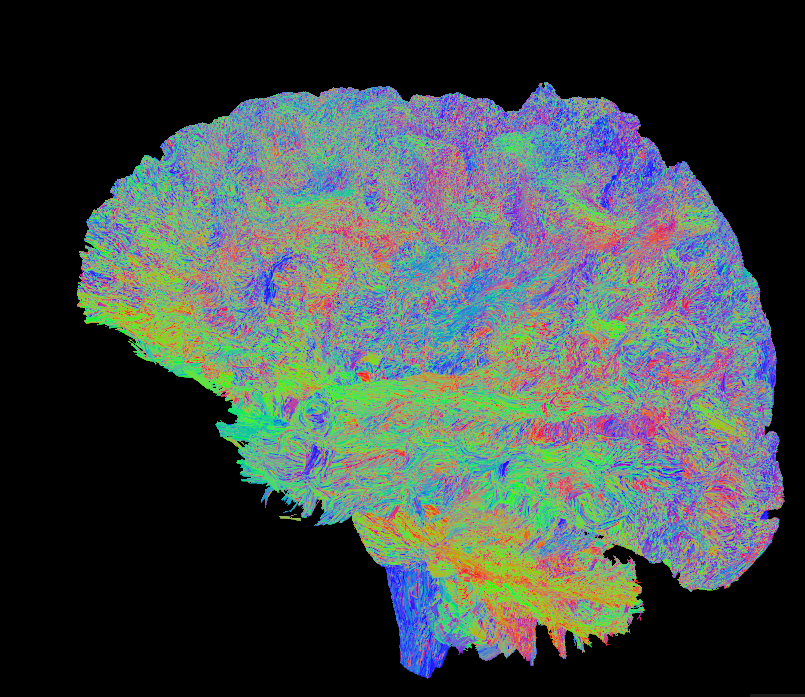
\includegraphics[height=0.9\textwidth,width=0.9\textwidth]{images/tractography.png}
         \caption{Tractography}
         \label{fig:1M_tract}
     \end{subfigure}
    \hfill
     \begin{subfigure}[b]{0.4\textwidth}
         \centering
         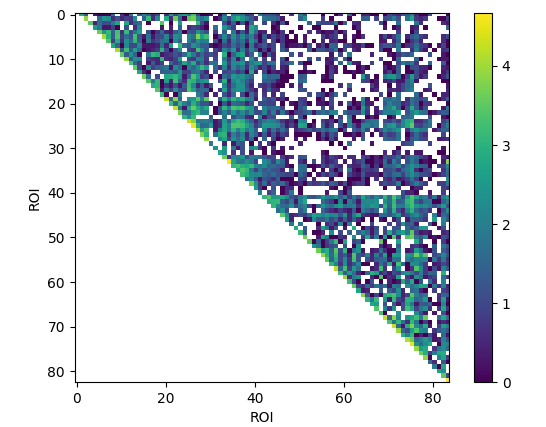
\includegraphics[height =0.9\textwidth,width=\textwidth]{images/connectome_1M.png}
         \caption{Connectome}
         \label{fig:connectivity_matrix}
        \end{subfigure}
    \vfill
        \begin{subfigure}[b]{0.6\textwidth}
         \centering
         \vspace{2em}
         %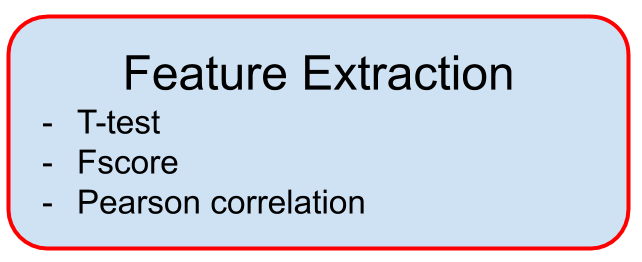
\includegraphics[height=0.3\textwidth,width=0.5\textwidth]{images/Features_1.png}
        \begin{tcolorbox}[box align= center,coltitle=black!75!black, colback=yellow!5!white,colframe=yellow!50!black,
  colbacktitle=yellow!80!black,title=\centering \large Feature Representation]
        \centering
        fscores, t-test, pearson correlation
        \end{tcolorbox}
        \caption{}
         \label{fig:feature extraction}
         \end{subfigure}
    \vfill
    \begin{subfigure}[b]{0.9\textwidth}
    \begin{subfigure}[b]{0.3\textwidth}
        \begin{tcolorbox}[coltitle=black!60!black ,colback=yellow!5!white,colframe=yellow!50!black,
  colbacktitle=yellow!75!black, fontupper=\color{black}, title=\centering \large Feature Selection]
        Select k\% features
        \end{tcolorbox}
         %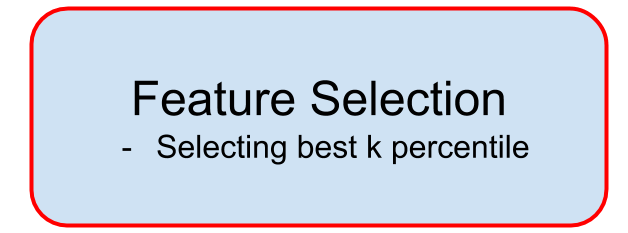
\includegraphics[height =0.8\textwidth,width=\textwidth]{images/Features_2.png}
         \vspace{+1.5cm}
         \label{fig:feature selection}
         \end{subfigure}
    \hfill
    \begin{subfigure}[b]{0.4\textwidth}
         \centering
         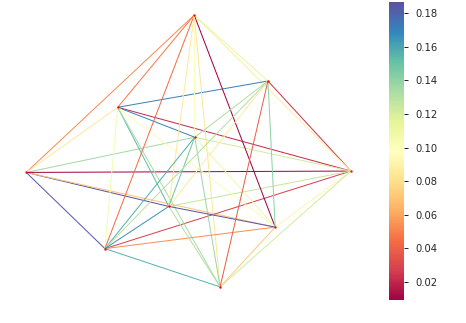
\includegraphics[height =0.8\textwidth,width=\textwidth]{images/mews.png}
         \label{fig:mewspip}
         \end{subfigure}
    \vspace{-2em}
     \caption{Parallel feature selection using baseline analysis and MEWS}
    \end{subfigure}
    \vfill
        \begin{subfigure}[b]{0.6\textwidth}
         \centering
         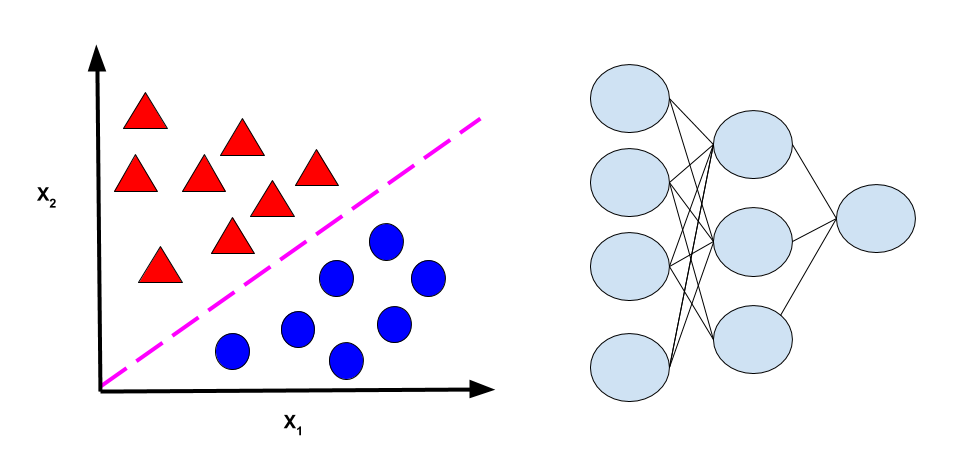
\includegraphics[height =0.4\textwidth,width=\textwidth]{images/classification.png}
         \caption{Classification}
         \label{fig:three sin x}
         \end{subfigure}
    \caption{(a) Whole brain tractography consisting of one million streamlines computed for each subject. (b) Connectivity matrix encoding DWI information. In this case, the matrix represents the number of streamlines between any two regions of interest in the $log_{10}$ scale. (c) Different statistical measures used to represent the importance of the original features present in the dataset.(d) Ranking used to determine the most important features which are then fed to the classifier. Parallelly, the MEWS is extracted from an input graph of statistical coefficients and is fed to the classifier (e) Classification using machine learning algorithms, such as SVMs, Random forests and MLPs.}
    \label{fig:pipeline}
\end{figure}

A classification task was designed for the MRI data from the Human Connectome Project. The pipeline consisted of four major steps. First, a whole brain tractography was generated on the basis of DWI scans for each subject. Second,  three types of connectomes were created for each subject and represented in the form of connectivity matrices. Thirdly, two different feature selection techniques were deployed for classification of subjects based on the connectivity matrices. Finally, machine learning classifiers were used to test the effectiveness of these two feature selection techniques. The summary of the pipeline is presented in \autoref{fig:pipeline}

The implementation of this pipeline was scripted in \textit{Python}. The preprocessing of the HCP data to generate tractography was done with the help of \textit{Mrtrix3} (\cite{tournier2019mrtrix3}).  Data was prepared in a classification ready format using \textit{Pandas} (\cite{pandas_2020}) dataframes. The Maximum Edge Weight Subgraph problem was implemented in \text{Java} based on a modification from \cite{DBLP:journals/corr/LobodaAS16} (\hyperlink{\textbf{github.com/ctlab/gmwcs-solver}}{https://github.com/ctlab/gmwcs-solver}). The final classification was based on machine learning from \textit{scikit-learn}(\cite{sklearn_2012}). 

\section{Data Acquisition}
\label{sec:acquisition}
Structural and Diffusion MRI for 203 subjects was acquired from the s900 release of the HCP (\cite{hcp2015wu}). Out of the total, 101 subjects were females and 102 were males. 83 females and 58 males were aged 26-30 and while the 34 males and 28 females were aged 22-25. The demographic information along with other markers about the subjects' emotion and cognition were obtained from the unrestricted access data available on \href{https://db.humanconnectome.org/}{\textbf{\textit{https://db.humanconnectome.org/}}}.

\subsection{Imaging data}
The structural and diffusion MRI files used for this project were obtained from the repositories containing volumes preprocessed using version 3 preprocessing pipelines of the HCP detailed in (\cite{GLASSER2013105}). A Siemens 3T Skyra system was used used to scan all subjects (starting in August 2012, housed at Washington University, St. Louis). The details of the acquisition protocol are mentioned in \cite{van2012human}.


There were two types of structural data required from the HCP pipeline for each subject in order to proceed with the task of the project. The first was a parcellation image consisting of a segmentation volume and a cortical surface parcellation based on the Desikan Killinay Atlas (\cite{desikan2006automated}), provided as a default in FreeSurfer). The second type was the T1w scan in subject space. This anatomical images was aligned to the location at the interface of hemispheres: the anterior commisure and posterior commisure (ACPC). It is a rigid body rotation so that the image gets 'centered', this process can be termed as registration.\iffalse This was a T1w volume data in the subject's native space obtained after rigid-body rotation to AC-PC alignment (rigidly aligned to the native axis of MNI space, also termed as registration )\fi. It was sampled at the same resolution as the diffusion data (1.25 mm isotropic, originally 0.77 mm isotropic).The parameters of the T1w images are presented in the \autoref{tab:structuralmri}.


\begin{table}[]
    \centering
    \begin{tabular}{|c|c|}
    \hline
         TR (ms) & 2400\\
    \hline
         TE (ms) & 2.14 \\
    \hline
         T1 (ms) & 1000 \\
    \hline
         Flip angle & 8 deg \\
    \hline
         FOV & 224x224 \\
    \hline
         Voxel Size & 0.77 mm isotropic \\
    \hline
    \end{tabular}
    \caption{Acquisition parameters for the structural image acquisition from the s900 release. }
    \label{tab:structuralmri}
\end{table}

\begin{table}[]
\centering
    \begin{tabular}{|c|c|}
          \hline
         Sequence &  Spin-echo EPI \\
          \hline
         slice thickness & 1.25 mm, 1.25 mm isotropic voxels\\
          \hline
         TR (ms) & 5520  \\
          \hline
         TE (ms) & 89.5 \\
          \hline
         Flip angle & 78 deg \\
          \hline
         Refocusing flip angle & 180 deg \\
          \hline
         FOV & 224 x 224 \\
          \hline
        Voxel Size & 0.77 mm isotropic \\
          \hline
        b-values & 100,2000 and 3000 s/mm^{2}\\
         \hline
    \end{tabular}
    \caption{Parameters for the acquisition of the Diffusion MRI data acquired from the HCP.}
    \label{tab:diffusionmripara}
\end{table}

\subsection{Label Preparation}
\label{sec:label_preparation}

\begin{table}
\label{table:personality}
\csvreader[
  tabular=|c*{5}{|c}|,
  table head=\hline Variable & Agreeableness & Openness &  Conscientiousness &  Neuroticism  & Extraversion\\ \hline,
  late after last line=\\\hline,
]{tables/personality_traits_summary.csv}{}%
{\csvcoli & \csvcolii & \csvcoliii & \csvcoliv & \csvcolv & \csvcolvi}

\caption{Summary of personality traits for all subjects.}
\end{table}

Their conversion to the classification task was as follows:
\begin{enumerate}
\item Record the median of the personality trait the training subjects
\item Divide the personality labels into 5 quartiles
 \item Remove the data of the subjects whose personality traits fall into the middle quartiles
 \item Binarize the variables such that the first two quartiles belong to the lower class and the last two quartiles correspond to the higher class
\end{enumerate}
Different types of labels were used to test the method
Personality traits are based on the five factor model of personality. The five different personality traits are Agreeableness, Conscientuousness, Neuroticism, Extraversion and Openness. They are often used in pyschology and pyschiatry to determine the behaviour of subjects
using questionnaires. The personality labels were continuous, their statistics in our dataset are depicted in \autoref{table:personality}.

The gender variables were categorical. For the classification task, male attribute was mapped to zero and females to one.


\section{Creating the Connectome}
\label{sec:creating_connectome}
\begin{figure}
    \centering
    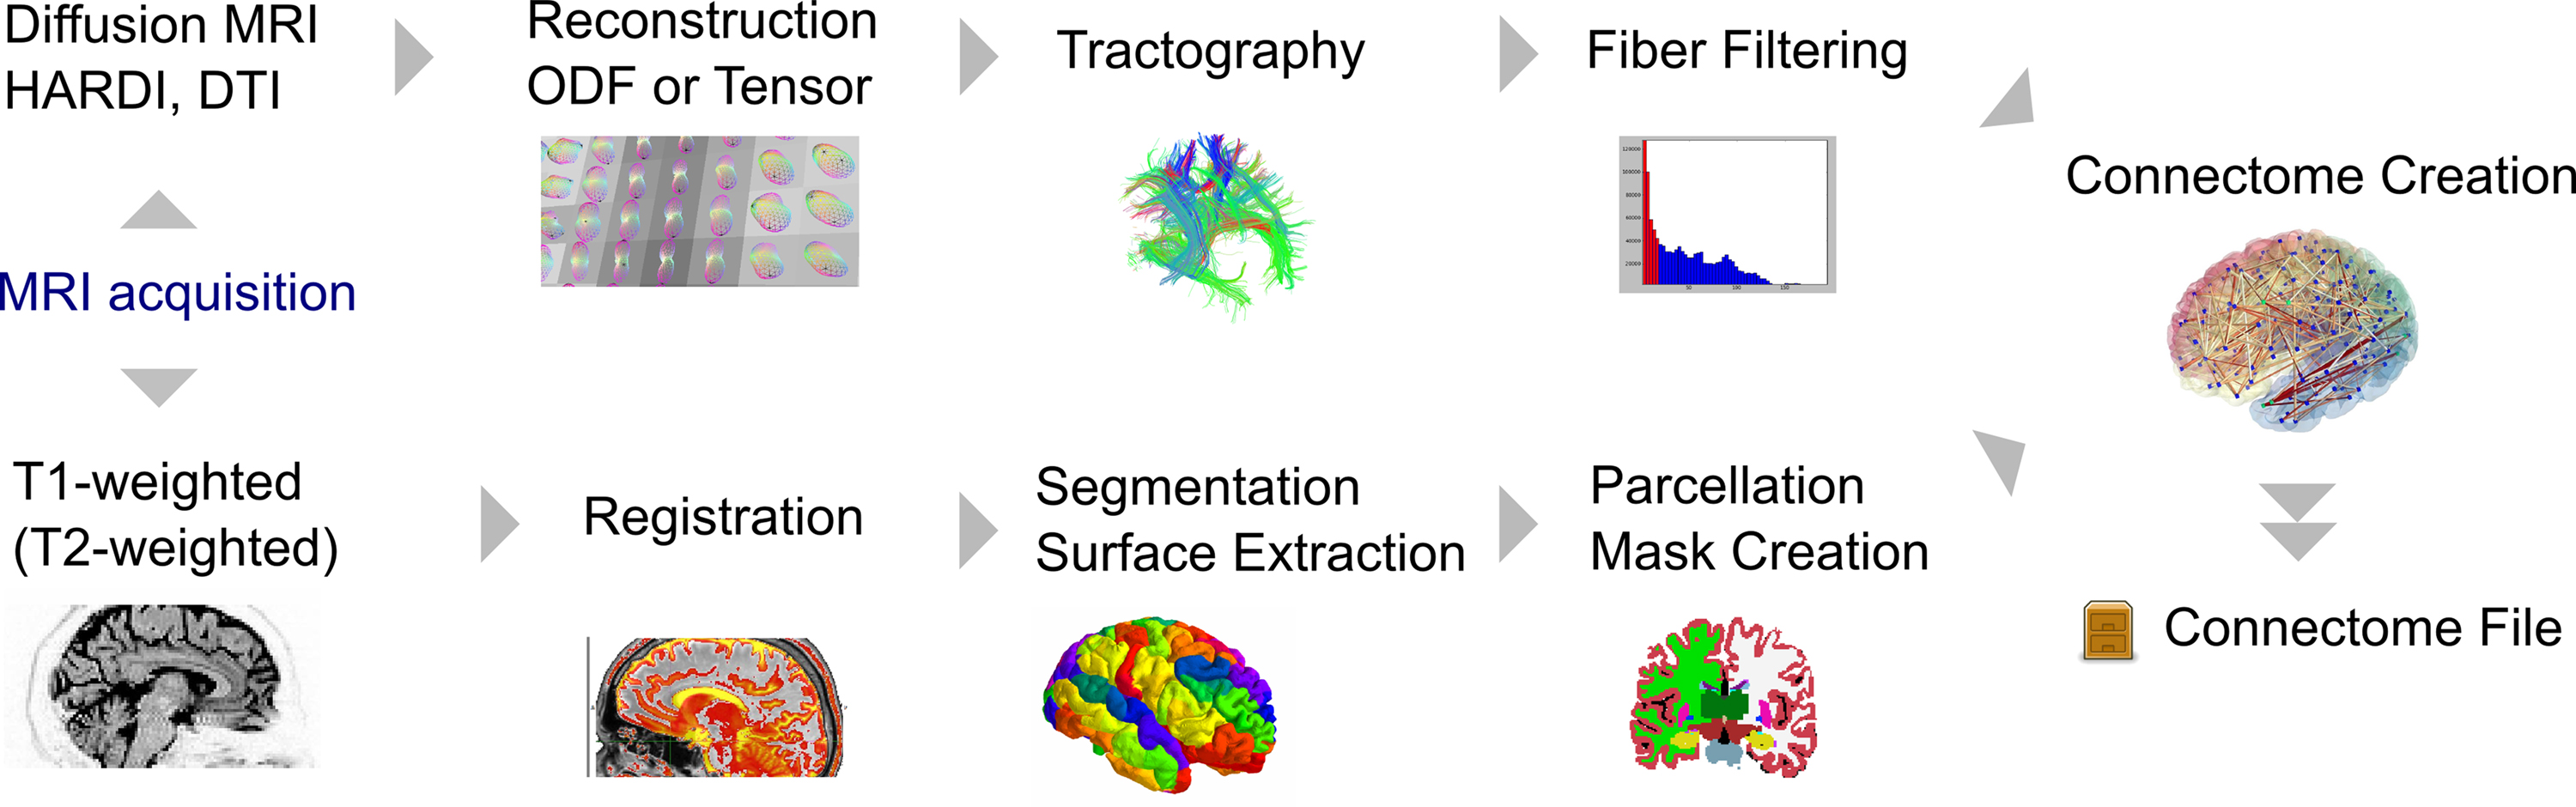
\includegraphics[width=\textwidth]{images/connectome_creation_workflow.png}
    \caption{Pipeline for creating the connectome for each subject. After the acquisition of the MRI data two parallel processes take place. The first parallel process is based processing the structural images for each subject in their native space. The second parallel process is the processing of the Diffusion data to generate Anatomically contstrained tractograms. After obtaining the fiber filtered tractograms and the parcellation masks with segmented tissues the connectome file is generated by determining the proprties of the streamlines that run between different ROIs. Image from \cite{gerhard2011connectome}}
    \label{fig:connectome_pipeline}
\end{figure}


For each subject, four types of DWI files were used. First, the preprocessed diffusion time series file. Second, the brain mask in diffusion space. The other two types were diffusion weighting and diffusion direction for each volume. The important characteristics of the dMRI images is that they obtained in very high resolution (1.25mm isotropic) using a Stejskal-Tanner (monopolar) diffusion encoding scheme as mentioned in \autoref{sec:DWI}. The q-space was sampled by including 3 shells at the b-values presented in \autoref{tab:diffusionmripara} with each gradient table defined by a single b-value acquired once with right-to-left and another in the opposite phase encoding polarities. 

For this project, the structural images from subject's native space were taken due to the nature of the tractography. Tractography is performed in the subject space since a structural image in this space is the best approximation of the subject's physical brain. 

A connectome was generated on the basis of tractography as explained in \autoref{sec:connectomics}.The pipeline was implemented on the basis of the tutorial on Structural Connectome for Human Connectome from the software package \textbf{\textit{Mrtrix3}}. The preparation of the structural connectivity matrices can be visualized in the figure \autoref{fig:connectome_pipeline}. This preparation mainly involves three steps which are explained in the following subsections.

The structural and diffusion images available within the HCP data were used to prepare the data for probabilistic whole-brain tractography (\cite{parker2003framework}). The parcellation image was used to generate a volume delineating locations of the nodes of the connectome for each subject while the T1w image in a subject's native space were used to generate a five-tissue type (5TT) segmented image.

\subsection{Structural Image Processing}
\label{subsec:struct_diff}

The first three steps of the structural image processing were readily accomplished by the HCP preprocessing pipeline. The segmentation surface was available from the HCP data as mentioned in \autoref{sec:acquisition}. However, the data obtained had a parcellation mask based on the default FreeSurfer segmentation which did not contain the numbering of the ROIs starting from 1. The parcellation mask was converted from FreeSufer's estimates of sub-cortical grey matter structures with the estimates from FSL's FIRST tool. This made the numbering of the ROIs (also the nodes in this case) from 1. 

In addition to creating the parcellation mass, a five tissue segmented image (5TT) was also generated. This was done on the basis of the T1w structural volume mentioned in \autoref{sec:acquisition} sampled at the same resolution as the diffusion data (1.25 mm isotropic). The 5TT image contained differentiation of brain regions into five tissue types, namely subcortical white matter, WM, cerebrospinal fluid (CSF) and optionally pathological tissue. The segmentation is based on FSL segmentation tools FIRST and FAST.This information about the location of different tissue types makes the tracking based on DWI images suitable for Anatomically constrained tractography.  (\cite{anattractsmith}). 


\iffalse
The diffusion image was first converted to a non-compressed format. The information about the diffusion gradient encoding was represented in the header of the file, the volume data was made continuous voxel-wise and the data points were converted to a floating point format. 
After this, the mean b=0 image was generated for visualization. The b=0 image serves as a sort of baseline for anatomical reference.

The multi-shell, multi-tissue response function was determined  in order to form Multi-Shell, Multi-tissue spherical deconvolution. 

Atleast three unique b-values are required to estimate three tissue comparments. These 

The deconvolution leads to the formation of a 4 dimensional image in which each 3D volume (as viewed in \comment{part of pipeline figure in preprocessing} is RGB encoded where the cerebrospinal fluid (CSF) is seen in red, the gray matter in green and the white matter in blue. 
\fi

\iffalse
In order to prepare for the tractography, the structural T1w images were preprocessed by Dr. Regina Wehler during the course of her master's thesis. At first the five-tissue-type images were generated using the 5ttgen fsl command. These are segmented 4D images whose fourth dimension represents 5 volumes containing the partial fractions of cortical gray matter, sub-cortical gray matter, white matter, CSF and pathological tissue. 
The input files were converted from the nifti to the mif format using the mrconvert command for the data to be compatible with \textbf{\textit{Mrtrix3}}. Then the 5TT images were generated using the 5ttgen fsl command -nocrop option to keep the images at the size of the original input. 
After obtaining the 5TT images, the segmentation from the original FreeSurfer format were converted to the scheme of the Desikan Killiany Atlas(\cite{desikan2006automated}) which divides the human cerebral brain into gyral based regions of interest.
\fi

\subsection{Diffusion Image Processing}
\label{sec:Diffusionimgprepro}
The first step of processing the diffusion images is to determine the fODF for probabilistic tractography. The fODFs were reconstructed using multi-shell, multi-tissue constrained spherical deconvolution (MSMT-CSD) based on the algorithm in \cite{jeurissen2014multi}. As mentioned in  \autoref{sec:highermodels} the CSD of response functions can determine the fODF distribution. Hence, CSD of the separate response functions from WM, GM and CSF was done in order to obtain the DWI signals of the three tissue types from the 5TT image.

The probabilistic whole-brain tractography of five-million fiber tracts was generated using \textbf{\textit{Mrtrix3}}. The streamlines were computed on the basis of the algorithm iFOD2 (\cite{tournier2010improved}). This algorithm uses the fiber orientation Distribution (fODF) image and determines candidate streamline paths (arcs), which have greater fODF amplitudes along the paths. By sampling the underlying fODF amplitudes along these arcs , it makes the streamlines likely to follow most probable paths.

Anatomical constraints on the tractography were provided using the five tissue type image. There were other series of constraints imposed in order to make the  tractography more informed. The seed points were dynamically determined using the Spherical-deconvolution informed filtering (SIFT) model \cite{smith2013sift} of the white matter fODFs. The cutoff value of 0.06 was set for FOD amplitude for terminating tracks. The maximum length of streamlines was set at 250 mm (200 times the voxel size) when the voxel size is 1.25mm. The tracking along a streamline was truncated if the fiber terminates at poor structural, then  retracking is performed. The streamlines were cropped whenever as the streamlines cross the grey matter-white matter interface. 

The tractography was then downsampled from five mullion fibers to one million fibers to preserve the most biologically relevant fibers using the SIFT algorithm (\cite{smith2013sift}). This provides more meaningful estimates of the structural connection density and also reduced the memory requirements. 
\iffalse
\begin{figure}
    \centering
    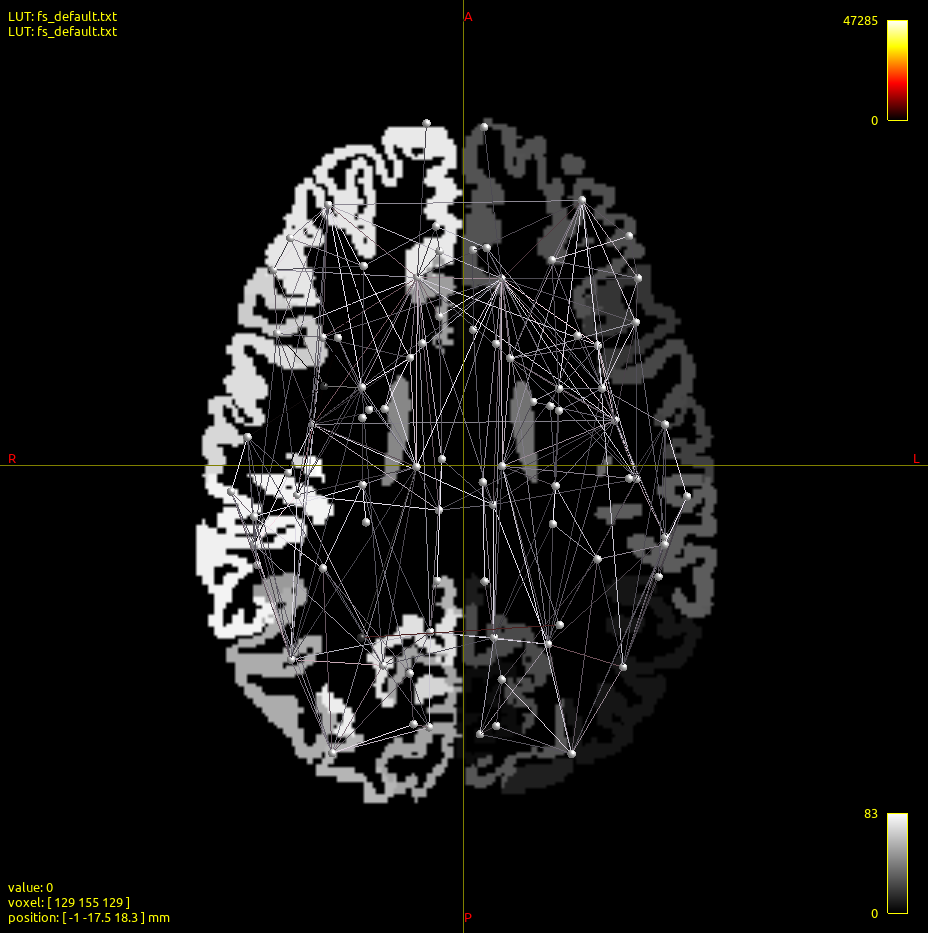
\includegraphics[width=0.8\textwidth]{images/connectome.png}
    \caption{Caption}
    \label{fig:connectome_vis}
\end{figure}
\fi
\subsection{Connectome Generation}
\label{subsec:connectomegeneration}
The connectome can be represented in the form of a graph as mentioned in \autoref{sec:connectomics}. After obtaining the streamline file and a parcellation image representing the subject specific node locations of the connectome, the connectome matrix was obtained in a \textit{.csv} format. It was generated from the whole brain tractography of one million tracts using 84 relevant grey matter parcellations (in \textit{\textbf{Mrtrix3}}) from the default FreeSurfer segementation specified by the Desikan Killiany Atlas. 

Using different parameter settings three types of features were extracted. The mean fractional anisotropy of the streamlines that connect the two regions (or mean FA, equation \autoref{eq:meanFA}). The average length of streamlines connecting two regions and number of streamlines between any two regions. The visualization can be seen in the \autoref{fig:connectivity_matrix}. The connectome is represented as an upper triangular matrix($84 x 84$) considering that the connections between two ROIs are symmetric.

\iffalse
In the  it can be seen that there is a need to decipher the streamlines which are terminating in the specified regions of interest
\fi
\section{Feature representation}
\begin{table}[]
    \centering
    \begin{tabular}{|l|c|c|}
        \specialrule{.2em}{.05em}{.05em}
         Type of feature & \multicolumn{2}{|l|}{Mean FA | Number of streamlines | Mean streamline length} \\
         \specialrule{.1em}{.05em}{.05em}
        \multirow{2}*{Feature Selection} & Solver & Baseline\\
        & Number of nodes & Percentage of features \\
        & [4...30]  & {2,5,10,50,100} \\
        \specialrule{.1em}{.05em}{.05em}
         Target labels & Personality metrics &  Gender\\
        \specialrule{.1em}{.05em}{.05em}
         Edge representations & pearson correlation coefficient &  t-test | fscores\\
         \specialrule{.1em}{.05em}{.05em}
     \end{tabular}     
    \caption{Parameters of the classification for different possibilities.}
    \label{tab:classify_combo}
\end{table}

Once the connectivity matrices for all the 201 subjects were computed and encoded in the format of a .csv file, a \textit{pandas} dataframe was prepared to serve as input to the classifier. Each row represented the data for an individual subject. Each column represented the connection between any two brain regions i.e. features in one cell of the connectivity matrix. Three different types of features obtained using the connectome files according to \autoref{subsec:connectomegeneration}. The design of the classification task was based on different attributes presented in \autoref{tab:classify_combo}. With one set of configurations for the two different techniques a classifier was trained for the solver based techniques as well as for the baseline experiments. The details will be discussed in the subsequent subsections.
\iffalse In the \textit{dataframe} be separate so that at any time only the same type of features are used to be filtered.The exact structure varied according to the feature selection techniques employed\fi. 

Self-loops were omitted from the analysis pipeline due to incompatibility with the solver based implementation and non-significant changes to classification accuracy based on the omission. Further, using the calculation of statistical coefficients on the raw data the importance of each feature was determined. 

The training set consisted of 141 subjects consisting of 83 females and 58 males aged 26-30. While the independent test set consisted of 34 male and 28 females aged 22-25. The data was standardized using \textit{sklearn} by removing the mean and scaling to unit variance since the different types of features were in separate scales of magnitude.


\subsection{Exclusion of self loops}
\label{sec:exclusion}
Self loops are considered the connections from the brain regions to themselves. They were excluded from the analysis before feeding to the classifier. Self loops were important consideration for the MEWS solver based implementation. Initially, the implementation from \cite{DBLP:journals/corr/LobodaAS16} was not functioning with input graphs that included connections from nodes to themselves. However, after removing such connections the MEWS implementation was able to solve the MIP formulation and produce subgraphs. It was required that the standard feature selection and MEWS based implementation be compared. There exclusion will be justified by the performance of the classifiers with and without the inclusion of self-connections between the ROIs. 

The importance of self loops was ascertained by seeing their effects on classification metrics. To evaluate their significance, a paired sample t-test was conducted. The first sample of the paired test is taken as the classification metric on the features with the self loops and the second sample excluding them. In general, the null hypothesis of a paired sample t-test remains that the differences between the observations from two samples is zero. Two slightly different experiments were carried out for classification of personality traits and gender. The formulas for calculation however remained the same. The t-statistic is calculated by:


\begin{align}
    \label{eq:pairedtest}
    t = \frac{\Tilde{X_{D}} - \mu_0}{\frac{s_{D}}{\sqrt{n}}} \\
    \Tilde{X_D} = \sum_{i=1}^{N} \frac{a_{i} - b_{i}}{n}
\end{align}where $s_D$ is the standard deviation of the differences between the metrics of the experiments with the self loops $a$ and without the self loops $b$. 

The null hypothesis for classification of personality traits was that the average of a particular classification metric on the basis of one feature (such as mean FA, mean streamline length and number of streamlines) is the same. The structure of the arrays $a$ and $b$ was the same.  There was one entry in the array for each possibility in a combination of choice for different attributes. The attributes were the five different personality traits, the percentage of features in the set $[2,5,10,50,100]$, and three different classifiers MLP, support vector machines, and random forest classifier one possibility of edge type. This corresponded to the $N=75$

In a similar fashion, the null hypothesis for the gender based classificaiton was the same. The structure of the arrays . The combination for each entry was the same except for the grouping of five different labels, here only one label was present that was the gender. and two different possibilities for the edges ( t-test and fscore). This resulted in $N=$30


The null hypothesis could not be rejected because for the test data, the p-values of these t-tests was high and hence not corresponding to any statistical significance. The results of this experiment are presented in \autoref{res:selfloops}. 
\iffalse
avg mean FA for all self loops(along all subjects in training data) 0.36
avg mean FA for all the other areas without the self loops (across all the subjects) is 0.345 (avg)
max avg mean FA in the range is 0.66 (in one connection avg along all subjects)
\fi

\subsection{Statistical Coefficients}
\label{subsub:statcoef}
\iffalse
Three different metrics were used to filter the features. Namely, pearson correlation coefficient, f-scores and the p-value of the t-test. The pearson correlation coefficient for the continuous values of the different personality traits, while the f-scores and t-test calculations were based on the conversion of the continuous variables into classes according to the \autoref{sec:label_preparation}. 
\fi
Statistical coefficients were determined to be one of the most important feature filter methods for the classification from Neuroimaging data. Filter methods were used since they do not compromise on interpretability of the results.

Three different statistical coefficients were used mainly. The first two were the t-test and the fscore, based on the discriminative power of a particular feature. The pearson correlation coefficient was used to determine the relationship between the continuous output variable values and the feature values. 

The fscore used in the analysis is used to measure how well the particular feature distinguishes between the two classes labelled as 1 and 2. It was calculated according to the equation \autoref{eq:fscores}. 

The t-test was processed in a different manner as compared to the first two metrics, the training data was divided into two groups, one belonging to class 1 and the other belonging to class 2. The null-hypothesis remained that the means of the given feature for the two samples are identical i.e. $\overline{x_{1}} - \overline{x_{2}} = 0$. The p-value of the t-test was used to determine it's statistical significance by converting it into the $log_{10}$ scale. Each p-value $p_x$ was represented by $ f(p_{x}) = (-1)*\log_{10} p_x$ so that a higher numerical value represents a higher statistical significance.



\subsection{Feature selection} 
The motivation to perform feature selection from considerations of time complexity and removal of redundant features. There were two types of feature selection techniques used before classification. The first one a classical feature selection technique based on statistical coefficients and is termed as the `baseline'. The second technique is based on extracting a subgraph after converting the original edge weights to statistical coefficients and is termed as the `solver' method based on the Maximum Edge Weight Subgraph problem (MEWS). 

The MEWS technique produces more interpretable results as compared to filter methods due to incorporation of graph topology. It is proposed due to the fact that analyzing the inter-subject differences at the subnetwork level is easier than analyzing dense subgraph of whole brain connectivity. 

\subsubsection{Baseline analysis}
% Question: which one do we report? Solver was working only with the pearson correlation coefficient.

Baseline experiments were solely based on the filter methods mentioned in \autoref{subsec:filtermethods}. In this technique, there is no information about graph topology or the biological correspondence of the data. Feature importance is determined purely on numerical values.

For each of the structural connections, the statistical coefficient was calculated based on the data and target variables from the training set. The metrics mentioned in \autoref{subsub:statcoef} were then used to rank the features. This ranking was based on first taking the absolute value of the coefficients and then dividing the coefficients for all features into a percentile distribution. This gave a ranking from which the top percentiles were selected according to a parameter $k \in \{2,5,10,50,100\}$. This parameter helped cover the trend of classifier performance as a function number of features.

\iffalse
The pearson correlation coefficient was computed between the values of the feature for the training subjects and their corresponding personality trait values. It was a trial to capture the linear relationship between a parameter (such as mean FA) representing a brain connection and the outcome label (i.e. personality trait).

The fscore based selection was done by computing the fscore between the feature values for the training set and thresholded values of the target variables according to the median of the training data labels. 

The fscores served as feature filtering step for the baseline experiments as they were used by dividing the f-score distribution into percentiles and then choosing the percentage of features we want in the specified top percentile. However, for the solver based experiments the fscores for each feature was (numerically) low which made the MIP problem hard to run computationally. Even multiplying the f-scores with an order of $10^3$ was not useful since the standard deviation of the f-scores was not too high (insert the standard deviation). 

This feature selection was in fact quite useful for the feature selection in the baseline experiments. The p-value of the t-test could be divided into percentile distributions and the top percentiles could be chosen accordingly. However, for the solver based experiments this selection did not work well due to computational effort. 

The pearson correlation coefficient in fact did work because it considers the linear nature of the personality trait coefficients. This type of feature selection is well reported in literature for Neuroimaging data considering continuous variables. It performed well for the baseline experiments as well as the solver based feature selection. For both the cases the absolute value of the pearson correlation coefficient was taken because only the correlation was important, whether it is positive or negative correlation was not a matter of concern for the analysis.

The f-score and the t-test were based on the binarization of the target variables according to the median values of the feature from the training set, this might lead to information loss and hence their lower numerical values. 
\fi

\subsubsection{Maximum Edge Weighted Subgraph}
\label{method:MEWS}

The special case of the MCWS (\autoref{sec:MEWS}), the MEWS was implemented because of no predefined node weighting for the regions of interest. The implementation was based on  the Java application from \cite{DBLP:journals/corr/LobodaAS16}. This application made use of the IBM ILOG CPLEX studio version 12.10 Java API. 

For each type of feature a separate graph was created specific to the target label of interest. The nodes in this graph consisted of 84 nodes defined by the cortical parcellations based on the Desikan Killiany Atlas. The edges were the connections between the ROIs weighted by the statistical coefficients calculated for the training data with respect to the target variables.

The nodes were given a constant negative weighting of $-0.01$ to assure a negative penality on the inclusion of an extra node. This made the conservation of a specified number of nodes alongside maintaining compatibility for MEWS  \autoref{eq:MEWS}. Additionally, sparsity to the input graph was introduced using two constraints. The first being that the absolute value of the edge weights shall not be zero and that features are conserved if and only if the tractography of each subject contains at least one streamline between the two nodes. 

\iffalse
Nodes could be given different types of weighting such as the maximum of the incoming edge weights, any numerical constant or the average of the incoming edge weights. Further the edges could be filtered on the basis of thresholds for the numerical features.
\fi

For creating the output graph, parts of the pipeline used in \cite{DBLP:journals/corr/LobodaAS16} were modified. Constraints mentioned in \autoref{sec:MEWS} were extended and the additional constraint was to preserve a specified number of nodes using
\begin{align}
    \label{eq:sum_constraints}
    \sum_{v=1}^{V} y_v = m        &&  \forall v \in V
\end{align}
where m is a controllable parameter specifying the number of nodes needed to be preserved in the output graph and $y_v$ is the binary variable mentioned in equation \autoref{eq:y_v}. The preprocessing module of the MCWS Java solver was disabled due to it's incompatibility with the required constraint \autoref{eq:sum_constraints}.

An object oriented approach was taken to implement a class derived from the \textit{networkx} (\cite{hagberg2008exploring}) for the different input graphs and their corresponding output graphs. At any time, the graphs created for a specific use case could be read from text files and their properties could be explored.

In order compare the features selected with this technique to the baseline experiments, it was important to infer the number of edges being preserved based on a specific input configuration. The output number of edges was then analyzed as function of the number of nodes. The results are presented in \autoref{fig:fun_num_edges}.


\section{Supervised Classification}

A Randomized Search 5 fold cross validation with implementation from \textit{scikit learn} was carried out for different algorithms in different cases based on the type of feature, the feature selection technique, target variables along with target labels are presented in \autoref{tab:classify_combo}. The cross validation was refitted using balanced accuracy on the test set. After the randomized search was finished, the best estimator was taken and fit to the training set. This classifier was then used to make predictions on an independent test set with difference in age range.

One model was trained each time there was a different configuration of settings presented in \autoref{tab:classify_combo}. The metrics used to assess classification performance were area under the curve, f1 score, accuracy and balanced accuracy.

The training set consisted of 141 subjects, 83 females and 58 males aged 26-30. The independent test set consisted of 62 subjects, 34 males and 28 females aged 22-25. The different age ranges for the training and the test set were chosen in to remove the confounding factors of age. Particularly when it came to personality traits which could be influenced by the age. If the training set consisted of different age ranges the algorithm could become biased by learning the age effects.


\section{Visualization}
Since the graphs included in the analysis for each subject were dense. It was important to design effective visualization techniques for intuitively interepreting the features selected by the baseline and solver based method. 

\subsection{Chord Diagram}
A chord diagram is an effective way of visualizing the flow between different nodes. The connectome containing the feature of the number of streamlines that connect any two ROIs was represented a chord diagram created with the help of package \cite{stevens2015holoviews}. Each ROI was represented as an entity or a fragment in the outer circle. The arcs drawn between the different node represent the connections and their thickness is proportional to the value of the number of streamlines in our case. 

In \autoref{fig:connectome_num_streamlines} the average number of streamlines (for all subjects) between any two regions are visualized. There are multiple arcs connecting the two regions and these arcs get bundled and result in a thicker arc. Similarly, the output graphs returned after the reduction from the solver is formed by determining the nodes and obtaining the group averaged number of streamlines between them. An example visualization is \autoref{fig:gender_num_strls_10}.


\end{document}

